
%----------------------------------------------------------------------------------------
%	PACKAGES AND OTHER DOCUMENT CONFIGURATIONS
%----------------------------------------------------------------------------------------

\documentclass[
10pt, % Main document font size
a4paper, % Paper type, use 'letterpaper' for US Letter paper
oneside, % One page layout (no page indentation)
%twoside, % Two page layout (page indentation for binding and different headers)
headinclude,footinclude, % Extra spacing for the header and footer
BCOR5mm, % Binding correction
]{scrartcl}

%%%%%%%%%%%%%%%%%%%%%%%%%%%%%%%%%%%%%%%%%
% Arsclassica Article
% Structure Specification File
%
% This file has been downloaded from:
% http://www.LaTeXTemplates.com
%
% Original author:
% Lorenzo Pantieri (http://www.lorenzopantieri.net) with extensive modifications by:
% Vel (vel@latextemplates.com)
%
% License:
% CC BY-NC-SA 3.0 (http://creativecommons.org/licenses/by-nc-sa/3.0/)
%
%%%%%%%%%%%%%%%%%%%%%%%%%%%%%%%%%%%%%%%%%

%----------------------------------------------------------------------------------------
%	REQUIRED PACKAGES
%----------------------------------------------------------------------------------------

\usepackage[
nochapters, % Turn off chapters since this is an article        
beramono, % Use the Bera Mono font for monospaced text (\texttt)
eulermath,% Use the Euler font for mathematics
pdfspacing, % Makes use of pdftex’ letter spacing capabilities via the microtype package
dottedtoc % Dotted lines leading to the page numbers in the table of contents
]{classicthesis} % The layout is based on the Classic Thesis style

\usepackage[top=1.25in, bottom=1.25in, left=1in, right=1in]{geometry} % dritchie: fix margins

\usepackage{arsclassica} % Modifies the Classic Thesis package

\usepackage[T1]{fontenc} % Use 8-bit encoding that has 256 glyphs

\usepackage[utf8]{inputenc} % Required for including letters with accents

\usepackage{graphicx} % Required for including images
\graphicspath{{Figures/}} % Set the default folder for images

\usepackage{enumitem} % Required for manipulating the whitespace between and within lists

\usepackage{lipsum} % Used for inserting dummy 'Lorem ipsum' text into the template

\usepackage{subfig} % Required for creating figures with multiple parts (subfigures)

\usepackage{amsmath,amssymb,amsthm} % For including math equations, theorems, symbols, etc

\usepackage{varioref} % More descriptive referencing


% dritchie: make paragraph spacing/indentation style nicer looking
\setlength{\parindent}{0em}
\setlength{\parskip}{1em}

%----------------------------------------------------------------------------------------
%	THEOREM STYLES
%---------------------------------------------------------------------------------------

\theoremstyle{definition} % Define theorem styles here based on the definition style (used for definitions and examples)
\newtheorem{definition}{Definition}

\theoremstyle{plain} % Define theorem styles here based on the plain style (used for theorems, lemmas, propositions)
\newtheorem{theorem}{Theorem}

\theoremstyle{remark} % Define theorem styles here based on the remark style (used for remarks and notes)

%----------------------------------------------------------------------------------------
%	HYPERLINKS
%---------------------------------------------------------------------------------------

\hypersetup{
%draft, % Uncomment to remove all links (useful for printing in black and white)
colorlinks=true, breaklinks=true, bookmarks=true,bookmarksnumbered,
urlcolor=webbrown, linkcolor=RoyalBlue, citecolor=webgreen, % Link colors
pdftitle={}, % PDF title
pdfauthor={\textcopyright}, % PDF Author
pdfsubject={}, % PDF Subject
pdfkeywords={}, % PDF Keywords
pdfcreator={pdfLaTeX}, % PDF Creator
pdfproducer={LaTeX with hyperref and ClassicThesis} % PDF producer
} % Include the structure.tex file which specified the document structure and layout

\hyphenation{Fortran hy-phen-ation} % Specify custom hyphenation points in words with dashes where you would like hyphenation to occur, or alternatively, don't put any dashes in a word to stop hyphenation altogether

% Switch font to helvectica (enclose in curly braces for local scope)
\newcommand*{\helvetica}{\fontfamily{phv}\selectfont}

%----------------------------------------------------------------------------------------
%	TITLE AND AUTHOR(S)
%----------------------------------------------------------------------------------------

\title{\normalfont\spacedallcaps{Daniel Ritchie}} % The article title

\author{\spacedallcaps{Research Statement}} % The article author(s) - author affiliations need to be specified in the AUTHOR AFFILIATIONS block

\date{} % An optional date to appear under the author(s)



\begin{document}

%----------------------------------------------------------------------------------------
%	HEADERS
%----------------------------------------------------------------------------------------

\pagestyle{scrheadings}
\clearscrheadings
\newcommand{\headertext}{\spacedlowsmallcaps{\color{black} Daniel Ritchie \color{halfgray} Research Statement}}
\ohead{\headertext}
\cfoot[\pagemark]{\pagemark}


\maketitle

My research focuses on solving complex procedural modeling and design problems using probabilistic programming. My work is interdisciplinary, sitting at the intersection of computer graphics, artificial intelligence, and programming languages. I believe in developing general-purpose solutions, rather than specialized fixes for one problem or application domain. This means that on the way to solving computer graphics problems, my work often leads to systems and algorithms that have broader impact for probabilistic programming and probabilistic inference in general.

In procedural modeling and design, content creators write programs that pseudo-randomly generate visual content, such as 3D models, websites, or arrangements of furniture. This approach allows designers to rapidly create and explore alternative design possibilities. It also scales to creating large amounts of diverse content without extensive human effort, which is becoming more important as the virtual worlds of films, games, and simulations grow larger and more detailed. Traditional procedural modeling tools operate via forward reasoning: the user writes a step-by-step recipe for generating content, such as a 3D model for a house. However, detailed, realistic content must also satisfy properties that are difficult to guarantee constructively---for example, the house models should be structurally stable. Satisfying such conditions seems to require \emph{inverse} reasoning, working backwards from the desired result.

Bayesian probabilistic inference provides a well-studied conceptual mechanism for this kind of inversion: the forward recipe serves as a generative prior distribution, and the desired properties can be encouraged via a likelihood function. Probabilistic programs are a natural choice for representing these types of distributions. They are a Turing-complete, universal family of probabilistic models, so they can capture the highly structured, recursive, mixed-continuous-discrete nature of many procedural models~\cite{Church}. They are also human-readable and human-writable and require little-to-no special expertise in probabilistic inference to author or understand.

Unfortunately, the expressiveness of probabilistic programs comes at a cost: inference on such complex programs is often intractable. We must resort to approximate methods that converge slowly, if at all. Thus, most of my work has focused on improving the reliability and runtime efficiency of probabilistic programming inference, with a particular eye towards procedural modeling applications in computer graphics. My research in this space has involved both algorithmic work (increasing the statistical efficiency of inference through new or improved algorithms) as well as systems work (making existing inference algorithms more computationally efficient).




% Following sections are all structured as: problem/opportunity, solution, result/impact

\section*{Eliminating redundant computation with C3}

The `Lightweight MH' variant of the Metropolis Hastings algorithm is a popular technique for implementing probabilistic programming inference~\cite{Lightweight}. It is easy to implement and can be embedded in an existing deterministic language, rather than requiring its own specialized interpreter or compiler. And it operates on arbitrary programs, including the complex programs found in procedural modeling and design applications. Unfortunately, it is also inefficient: every Metropolis Hastings proposal triggers a complete re-execution of the program, despite the fact that the proposal often only changes a small subset of the program's execution trace. Probabilistic languages that run on custom interpreters often exploit this fact for faster inference, but they are complicated to implement and do not integrate as readily with existing deterministic code.

To get the best of both worlds---efficient, incrementalized proposals in a lightweight, embedded system---I developed a new MH implementation technique called C3~\cite{C3}. C3 leverages two insights. First, it transforms programs into continuation passing style (CPS): this makes continuations available at every point in the program, so execution can resume from anywhere. Second, C3 caches the receiver, inputs, and output of each function call, since many calls can be skipped when these quantities have not changed.

C3 significantly accelerates MH proposals. In the procedural modeling example below, where a tree-generating program is encouraged to take the target shape on the left, C3 runs nearly 10 times faster than Lightweight MH. Its two components, caching and CPS, work synergistically, delivering greater speedups when used together than the sum of their individual contributions. C3 also works well for many latent variable models in Bayesian data analysis, delivering 20-100x speedups on hidden Markov models, Gaussian mixtures, topic models, and hierarchical regression models. C3 is publically available as the \texttt{IncrementalMH} inference method in the open-source WebPPL programming language~\cite{WebPPL}.

\vspace{1em}
\begin{figure}[h!]
\centering
\setlength{\tabcolsep}{2pt}
\begin{tabular}{ccc}
	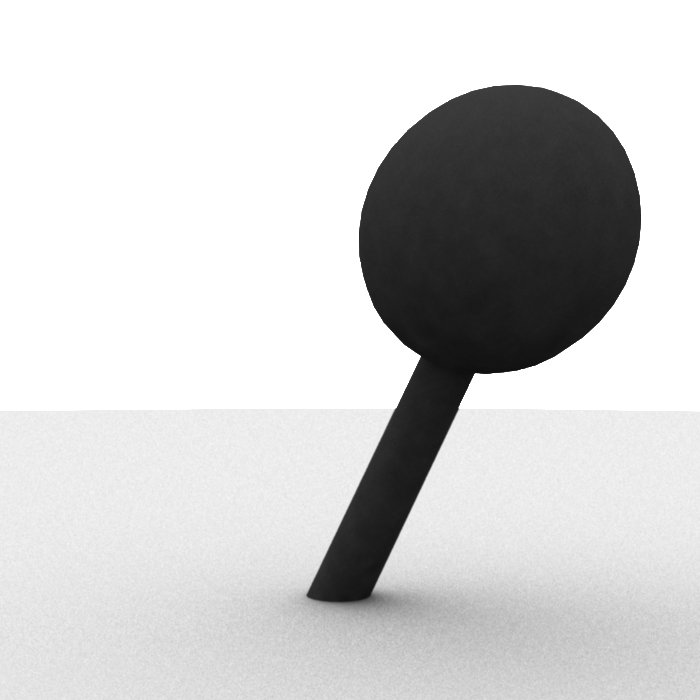
\includegraphics[width=0.25\linewidth]{figs/c3/target} &
	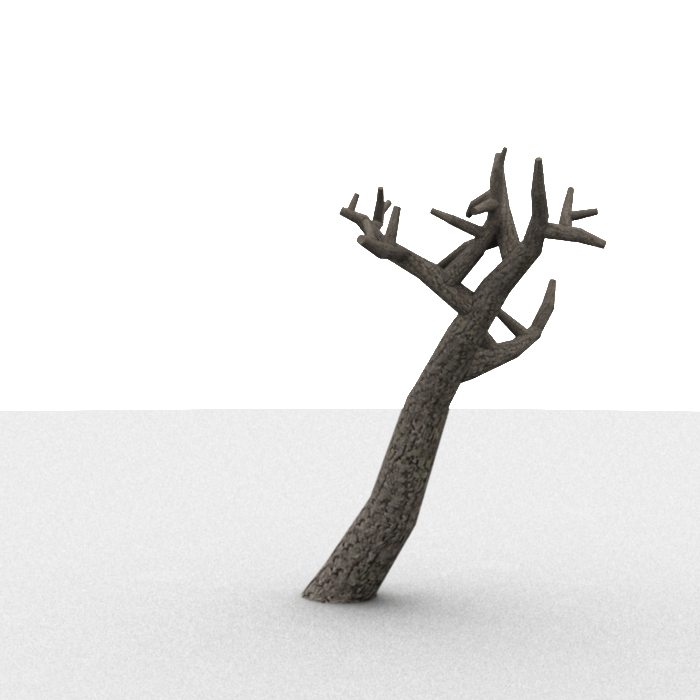
\includegraphics[width=0.25\linewidth]{figs/c3/result} &
	\shortstack{ 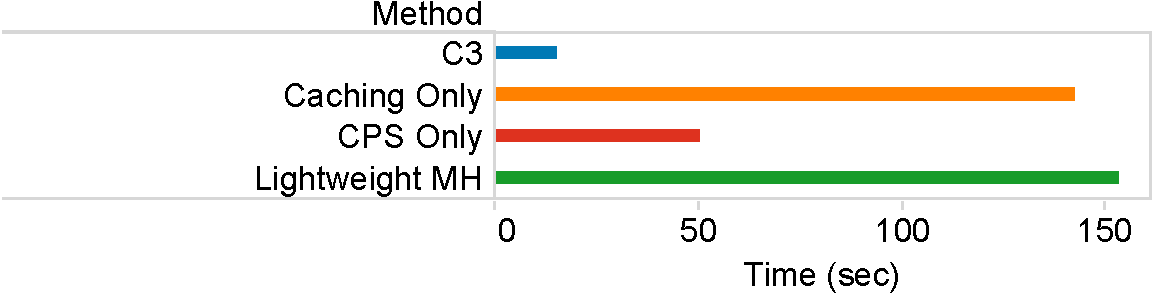
\includegraphics[width=0.5\linewidth]{figs/c3/procmod_time} \\ 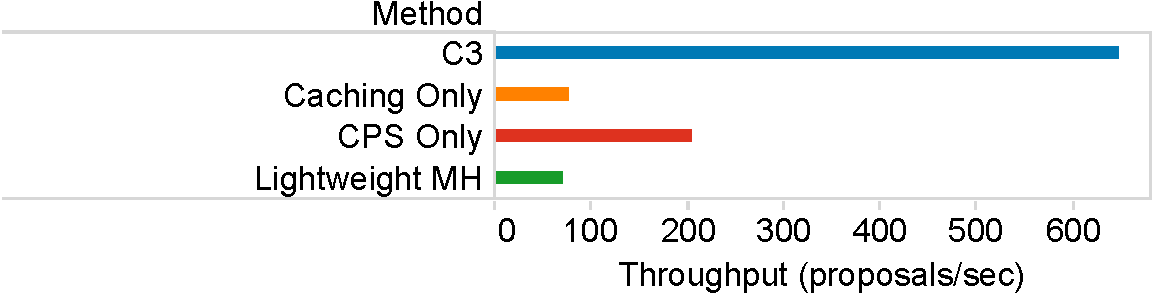
\includegraphics[width=0.5\linewidth]{figs/c3/procmod_throughput} } \\
	{\helvetica \scriptsize{Target}} & {\helvetica \scriptsize{Output}} & 
\end{tabular}
\end{figure}



\section*{Dealing with tight constraints using HMC}

Lightweight MH is a `single-site' Metropolis Hastings algorithm: it proposes changes to one random variable at a time. This strategy can break down when faced with likelihoods that induce tight constraints between multiple variables. For example, constraining the interior volume of a procedurally-generated bottle couples every random variable in the program. Changing one variable without also performing a corresponding change to the others leads to a change in volume and thus a drop in likelihood, so Lightweight MH struggles in these situations. Some programs admit problem-specific multi-variable proposal strategies to get around this issue: in the bottle example, cross-sections of the shape could be carefully adjusted in pairs to preserve volume. But these strategies can be difficult to discover and design, and they do not generalize to new problems.

In my work, I recommend using Hamiltonian Monte Carlo (HMC) in such situations instead~\cite{GraphicsHMC}. HMC simultaneously proposes changes to multiple continuous variables; these proposals stochastically follow the probability \emph{gradient}, increasing the chance that they will result in a high-probability state. The necessary gradient can be derived computationally using automatic differentiation, so it need not be written explicitly by the programmer. These properties make HMC an attractive, general-purpose candidate for inference in tightly-constrained procedural models.

I have shown that HMC successfully generates design suggestions in two different domains: constrained vector art coloring and stable stacking structures. The figure below shows several stable variations on a complex arch-like structure that HMC discovered, despite the tight global constraint introduced by encouraging structures to be in static equilibrium (Left). By contrast, Lightweight MH quickly becomes stuck in the first stable configuration it finds (Right). The source code for these examples is available online, and the underlying HMC implementation is part of Quicksand, my open-source system for high-performance probabilistic programming~\cite{Quicksand}.

\vspace{1em}
\begin{figure}[h!]
	\centering
	% \setlength{\tabcolsep}{2pt}
	\begin{tabular}{ccc|c}
		\raisebox{-.5\height}{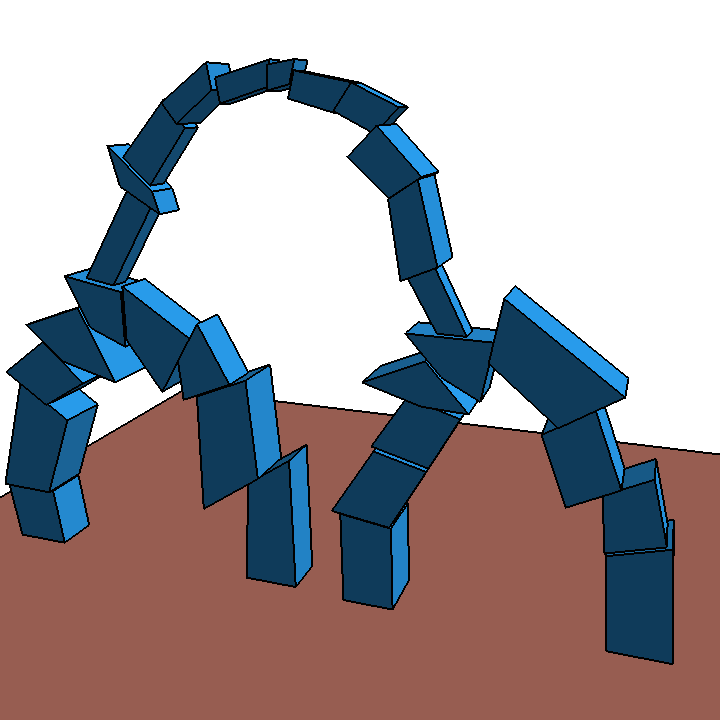
\includegraphics[width=0.23\linewidth]{figs/hmc/hmc_1.png}} &
		\raisebox{-.5\height}{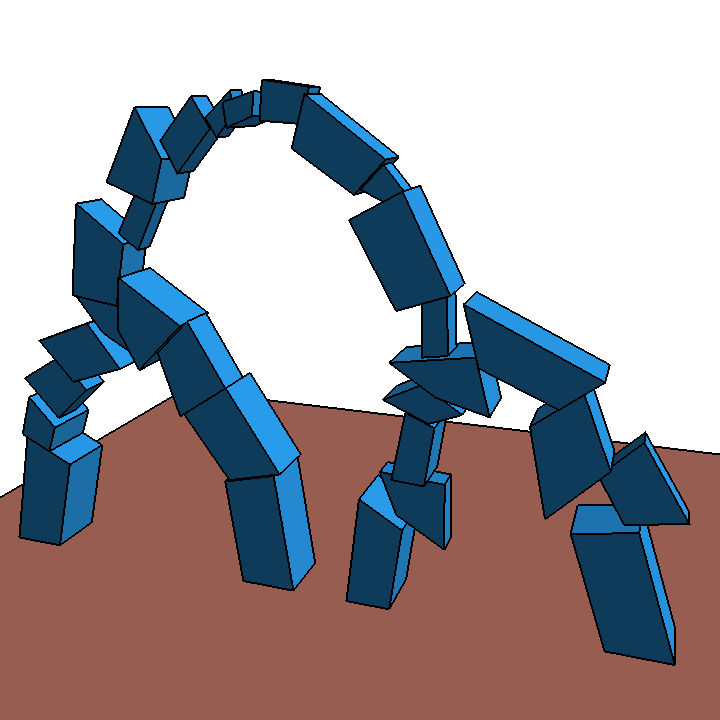
\includegraphics[width=0.23\linewidth]{figs/hmc/hmc_2.png}} &
		\raisebox{-.5\height}{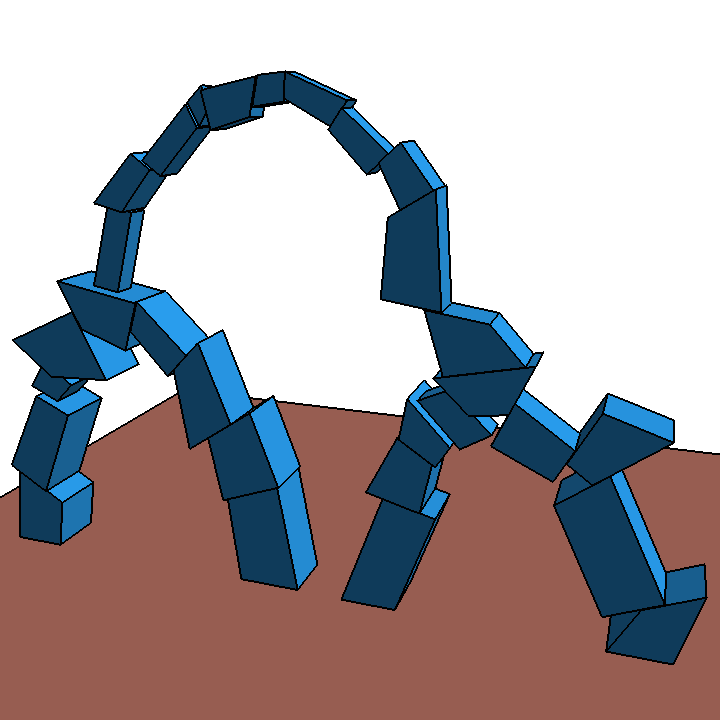
\includegraphics[width=0.23\linewidth]{figs/hmc/hmc_3.png}} &
		\raisebox{-.5\height}{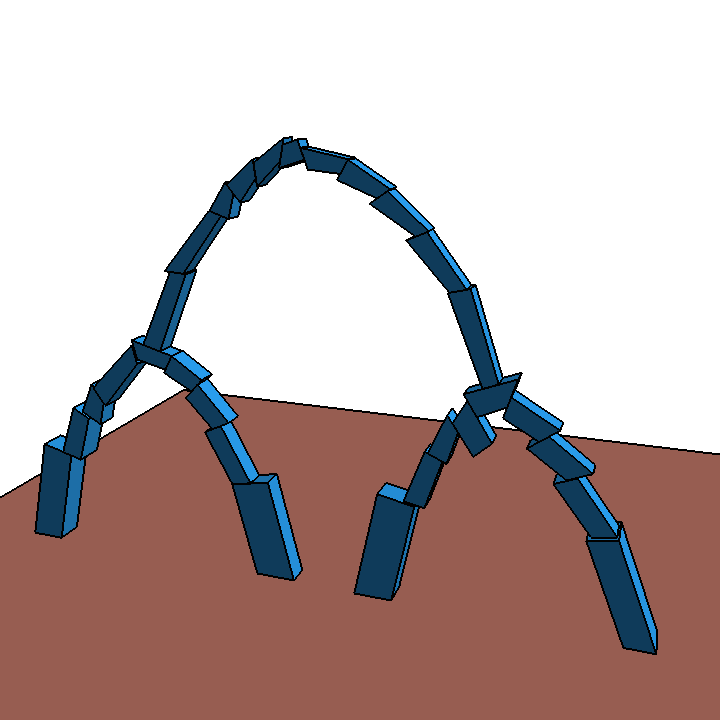
\includegraphics[width=0.23\linewidth]{figs/hmc/mh.png}} \\
		\multicolumn{3}{c}{{\helvetica \scriptsize{HMC Samples}}} & {\helvetica \scriptsize{MH Sample}}
	\end{tabular}
\end{figure}



\section*{Handling branching structure with SOSMC}

Motivate by talking about how MCMC gets stuck in structural local maxima, how SMC could avoid that problem entirely. Inspired by recent work adapting SMC to probabilistic programs. Have to handle `non-linear' programs with structured branching, as well as transdimensionality. Have to linearize call tree. Linearization affects SMC performance. Development of SOSMC. Stochastic future. Cool results.




\section*{Future research agenda}

Opening statement about how PPLs for design is a field in its infancy, lots of open sky to explore. Opportunities to integrate insights from both AI/ML and PL/compilers into computer graphics and design tools is very exciting.

Making inference more real-time (mention some cool examples of real-time constrained content generation that we'd like to achieve). Talk about amortized inference as an idea. Specifically talk about variational inference as a mechanism for achieving it. Mention/cite recent work in using neural networks to build recognition models. But need further work to make these work with structure-changing models, and with constraints not derived from data.

Inference is too much a `batch operation'---we need to account for the presence of the human user. More interactivity. Programs should react to user input / new data; FRP ideas. Also, mixed-initiative (or is the phrase I'm looking for mixed-modality?) programming, where user sometimes writes code and sometimes specifies examples / does direct manipulation, and the system infers code from that interaction.

Exploring connections to nearby disciplines. Procedural models as structured priors for computer vision, 3D reconstruction. Can also be viewed as a form of `content creation by scanning the world.' Also, real-time inference has other applications in time-constrained / resource-limited environments. Examples include building programmable embedded systems for doing sensing/inference. Would be useful in robotics, also just as a DIY thing for people to put around their houses, etc.


\bibliographystyle{plain}
\bibliography{research}


\end{document}


